\documentclass[Afour,sageh,times,doublespace]{sagej}

\usepackage[utf8]{inputenc}
\usepackage[T1]{fontenc}
\usepackage{moreverb,url}
\usepackage{graphicx}
\usepackage{amsmath,amssymb}
\usepackage{booktabs,longtable,array,calc}
\usepackage{newunicodechar}
\newunicodechar{ρ}{\ensuremath{\rho}}
\newunicodechar{−}{\ensuremath{-}}
\newunicodechar{∞}{\ensuremath{\infty}}
\newunicodechar{×}{\ensuremath{\times}}
\newunicodechar{≈}{\ensuremath{\approx}}
\newunicodechar{≤}{\ensuremath{\le}}
\newunicodechar{≥}{\ensuremath{\ge}}
\newunicodechar{∈}{\ensuremath{\in}}
\newunicodechar{Σ}{\ensuremath{\sum}}
\newunicodechar{λ}{\ensuremath{\lambda}}
\newunicodechar{η}{\ensuremath{\eta}}
\newunicodechar{Ψ}{\ensuremath{\Psi}}
\newunicodechar{κ}{\ensuremath{\kappa}}
\newunicodechar{γ}{\ensuremath{\gamma}}
\newunicodechar{τ}{\ensuremath{\tau}}
\newunicodechar{σ}{\ensuremath{\sigma}}
\newunicodechar{Ω}{\ensuremath{\Omega}}
\newunicodechar{≠}{\ensuremath{\neq}}
\newunicodechar{→}{\ensuremath{\to}}
\newunicodechar{∼}{\ensuremath{\sim}}
\newunicodechar{²}{\ensuremath{^{2}}}
\newunicodechar{–}{--}
% pandoc-fragment helper macros (this file is assembled without pandoc's template)
\providecommand{\tightlist}{\setlength{\itemsep}{0pt}\setlength{\parskip}{0pt}}
\providecommand{\real}[1]{#1}
\providecommand{\pandocbounded}[1]{#1}
\usepackage[colorlinks,bookmarksopen,bookmarksnumbered,citecolor=red,urlcolor=red]{hyperref}

\graphicspath{{costly_selective_closure_supplement/figures/}}

\begin{document}

\runninghead{Zhang}

\title{Costly Selective Closure: A Comparative Heuristic for Life-Likeness in Artificial Systems}

\author{Yuxin Zhang\affilnum{1}}

\affiliation{\affilnum{1}Independent Researcher}

\corrauth{Yuxin Zhang, Independent Researcher.}

\email{zyx1st@gmail.com}

\begin{abstract}
Artificial life lacks a widely shared operational grammar for comparing degrees of life-likeness across substrates. Existing markers --- metabolism, autopoiesis, adaptive behavior, predictive closure --- each capture part of the target, but they blur the difference between systems that merely update and systems that must sustain an organized mode of existence. This paper develops a comparative, substrate-neutral heuristic: life-likeness is a matter of degree in \textbf{costly selective closure}, read along four coupled dimensions --- selective bandwidth (\(d\)), maintenance cost (\(\Psi_f\)), hysteretic memory (\(\eta\)), and irreversible vulnerability (\(V\)). Together these distinguish passive from active closure and make token-level irreversibility central to the boundary between buffered simulation and stake-bearing organization.

We then isolate one dimension experimentally. Two independent reinforcement learners face an identical survival dilemma that differs in a single variable: whether energy depletion terminates the agent (real stake) or cheaply resets it (buffered stake). Under a matched reward function, only the real-stake regime stabilizes costly cooperation after the explicit incentive is withdrawn --- post-withdrawal mutual cooperation of \textbf{0.55 versus 0.04} across \textbf{30 seeds} (\(p < 0.0001\)). The effect survives removing the death penalty entirely, holds across a payoff sweep, and forms a monotone dose-response as the maximum number of lives increases from one to unbounded.

These results isolate the causal role of token-level irreversibility; they do not validate the full four-dimensional framework. What the paper offers is a buildable, comparative heuristic for probing when artificial systems sustain genuinely life-like commitments --- not a definition of life.
\end{abstract}

\keywords{costly selective closure, life-likeness, artificial life, token irreversibility, vulnerability, reinforcement learning, adaptive agency, active closure}

\maketitle

\subsection{1. Introduction}\label{introduction}

Artificial life has always been both a technical program and a philosophical method. Instead of asking only what life is in the abstract, it asks what must be built, varied, and maintained for something life-like to appear. The question is therefore not only classificatory. It is operational: what should count as a success condition for artificial life?

This remains unsettled. Different traditions emphasize different signatures. Self-reproduction captures evolutionary open-endedness but excludes sterile organisms and many familiar living phases. Metabolism captures energetic organization but risks including fire. Autopoiesis captures self-producing organization and organizational closure (Maturana and Varela, 1980), but is often difficult to compare across substrates (Moreno and Mossio, 2015). More recent frameworks based on predictive processing or active inference highlight adaptive regulation and boundary maintenance, but by their generality they can blur the difference between organisms, thermostats, and highly capable digital agents. The present proposal also sits alongside work on minimal autonomous systems, enactive artificial intelligence, and recent basal-cognition approaches that treat cognition and life-like agency as graded across phylogeny (Ruiz-Mirazo et al., 2004; Froese and Ziemke, 2009; Lyon et al., 2021; Lyon and Cheng, 2023). It is also sympathetic to Thompson's life-mind continuity thesis, while departing from it in treating organizational closure as necessary but not by itself sufficient for stronger forms of life-likeness (Thompson, 2007).

For artificial life, this creates a practical problem. Without a shared operational grammar, systems with very different organizational profiles are often discussed in the same vocabulary of ``adaptation,'' ``agency,'' or ``self-maintenance.'' We can describe Conway patterns, Lenia morphologies, soft robots, language models, and bacteria as exhibiting some kind of organization, but not all organization is equally life-like. What is needed is a comparative grammar broad enough to compare unlike systems while still sharp enough to distinguish mere update from consequential self-maintenance.

This paper develops a substrate-neutral operational hypothesis: life-likeness increases when an organized process must maintain selective closure under non-trivial cost, retained history, and consequential failure. The proposal is stated in a self-contained way and does not depend on any broader metaphysics. A life-like system, on this view, is not merely one that persists, computes, or reproduces. It is one that:

\begin{enumerate}
\def\labelenumi{\arabic{enumi}.}
\tightlist
\item
  selectively couples to a non-trivial portion of its world,
\item
  pays a non-zero cost to maintain that coupling,
\item
  carries the effects of past selections forward in memory and structure, and
\item
  faces meaningful consequences if its regulation fails.
\end{enumerate}

The point is not to introduce a new essence of life. It is to give artificial life a buildable discrimination rule. On this view, life-likeness is a gradient rather than a binary threshold. Systems can be more or less life-like depending on the degree to which they exhibit selective bandwidth, maintenance cost, hysteresis, and vulnerability. These four dimensions are offered as a four-dimensional comparative heuristic rather than a definition; the controlled experiment reported below (Section 4.5) isolates the causal role of just one of them, token-level irreversibility (\(V\)), and leaves the joint validation of all four as open work.

\subsection{2. Why Existing Criteria Stop Too Early}\label{why-existing-criteria-stop-too-early}

Classical definitions of life usually succeed by being locally right and globally incomplete. Reproduction identifies one important route by which life persists through time, but not all living systems are reproducing at every moment, and many life-like artifacts may never reproduce at all. Metabolism captures energetic openness and thermodynamic work (Schrödinger, 1944), but by itself it says too little about selectivity or organization. Autopoiesis comes closer by focusing on self-producing organization, yet its explanatory strength can become a weakness when researchers need tractable comparisons across different media.

The same problem appears in more recent discussions of adaptive systems. A system can maintain a boundary, minimize error, or stabilize a policy without this being enough to make it meaningfully life-like. A thermostat is organized, robust, and responsive. A large language model can exhibit astonishing behavioral complexity. A reinforcement-learning agent can maximize reward under changing conditions. Yet there remains an intuitive and theoretical difference between systems that merely implement a designer's structure and systems whose way of existing is itself under stake.

The missing distinction is between \textbf{update} and \textbf{consequential self-maintenance}.

Many systems update. Far fewer must continuously pay to remain what they are. In ordinary biological cases, failure has non-trivial consequences: the organism exhausts energy, loses integrity, suffers damage, or dies. Its regulatory activity therefore has existential weight. By contrast, many computational systems operate under extensive buffering. They may be reset, copied, restored, paused, or run again with little cost to their identity. They can display goal-directed behavior without bearing much of the burden that makes biological regulation matter.

Artificial life needs a comparative measure that can register this difference without collapsing into substrate chauvinism. It should not require carbon chemistry. But neither should every well-regulated or behaviorally rich system be treated as equally life-like. The question is not whether a system behaves as if it had a world. The question is whether it must selectively construct and maintain such a world under real cost and consequence.

This also clarifies the relation to active inference. Active inference provides a powerful account of adaptive regulation under a Markov blanket, but by design it does not distinguish between systems that maintain that blanket at negligible cost to themselves and systems for which boundary-maintenance is existentially burdensome (Friston, 2013; Kirchhoff et al., 2018). For a broader survey of mathematical approaches to agents, many of them predating active inference, see Baltieri and Suzuki (2025). Recent analyses of the free-energy principle (FEP) in concrete stochastic systems, and recent critiques of blanket-based generalization, reinforce the point that broad descriptive coverage does not by itself settle what kind of organized system is under study (Raja et al., 2021; Aguilera et al., 2022). The present framework adds that distinction through the vulnerability dimension \(V\): two systems may be equally well-described by active inference while differing sharply in life-likeness if one can be freely reset and the other cannot. What \(V\) adds is therefore not the generic idea that systems resist dispersion. FEP already captures that descriptive insight. The added claim is about token-level irreversibility: whether failure is borne by the individual system whose organization is at issue, or whether loss is cheaply externalized and reversed by the surrounding setup.

A natural objection arises: does \(V\) simply reintroduce a subtler form of chauvinism by favoring media with irreversible physical loss? The framework's answer is no. It does not privilege carbon, metabolism, or any specific material substrate. What it requires is that the continued organization of the token system be non-trivially at stake. In principle, a digital system could satisfy this condition if its persistence were bound to local irreversible processes rather than to cheap perfect restoration. A simple thought experiment would be an embodied digital agent tied to aging edge hardware with no maintained backup, or an irrevocable smart-contract agent whose local state transitions cannot be rolled back without destroying the token process under evaluation. What is excluded is not digitality as such, but architectures in which losses are systematically externalized and undone by design.

A deeper objection targets the biological relevance of token-level irreversibility. In evolutionary biology, what is conserved is often information at the level of the lineage or population, not the individual organism; a population of adequate size supplies precisely the kind of cheap backup that the framework treats as reducing life-likeness, and suicidal altruism seems to show that the token organism is dispensable while only the information matters. Two replies are needed. First, the present claim is deliberately about the token organized system, not about the unit of selection. Whether a lineage is buffered is orthogonal to whether a particular organized process bears the cost of its own maintenance: the redundancy of a species does not make an individual bacterium's self-production any less costly, nor its failure any less terminal for that bacterium. The framework grades the life-likeness of the token that maintains itself and stays silent about which units evolution optimizes. Second, and conceding part of the objection, the framework does not require that irreversibility be learnable by the token from its own destruction. A system need not, and generally cannot, learn from its own death. The claim is weaker and testable: whether failure is token-terminal or cheaply reversible changes the selective pressure on an organized process, even when that pressure is applied across many trials rather than experienced within a single life (Watson and Szathmáry, 2016). Section 4.5 exhibits exactly this structure. The pressure that stabilizes costly self-maintenance is exerted across a population of episodes, yet what it settles on depends entirely on whether each episode's failure is terminal. Token-level irreversibility is therefore not merely an observer's relabeling of otherwise identical dynamics: in the controlled setting of Section 4.5 it acts as a control variable that reshapes what an adaptive process settles into. This is a limited result in one environment, not a refutation of the units-of-selection view; it shows only that reversibility is doing causal work there rather than being an inert redescription.

\subsection{3. Costly Selective Closure}\label{costly-selective-closure}

\subsubsection{3.1 Selective Construction}\label{selective-construction}

The proposed framework begins with a simple thought: every candidate system faces a space of possible states, perturbations, and interactions. Life-like systems do not passively occupy this space. They selectively stabilize a small and usable region of it.

It is helpful to name three things: the open \textbf{possibility space} available to a system, its currently \textbf{maintained state}, and the relatively stable \textbf{retained constraints} sedimented by prior successful selection. The substantive point is simply to distinguish possibility space, current organization, and retained constraint.

Let \(\Omega_t\) denote the system's currently accessible possibility space and \(x_t\) its maintained state. We can write the next state schematically as

\[
x_{t+1} = (1 - \eta)\,\hat{G}_{\theta}[\Omega_t] + \eta x_t
\]

where \(\hat{G}_\theta\) is a selection-update operator and \(\eta \in [0,1]\) is a hysteresis term. The equation is intentionally minimal. It says only that current organization depends partly on present selection and partly on retained structure from the past. When \(\eta = 0\), the system is purely reactive. When \(\eta > 0\), previous selections constrain current ones.

This process can be called \textbf{selective construction}: a system does not encounter all possible states equally, but compresses possibilities into an actionable world. In artificial systems, the same question can be posed constructively: what dimensions does the system track, what does it ignore, and what does it take to keep that selection stable?

\subsubsection{3.2 Four Dimensions}\label{four-dimensions}

The degree of life-likeness is evaluated along four coupled dimensions.

\textbf{Selective bandwidth (\(d\)).} This is the effective dimensionality of the system's selective coupling to its environment. One convenient formalization is the effective rank of the operator's spectrum:

\[
d = D_{eff}(\hat{G}) = \frac{(\sum_i \lambda_i)^2}{\sum_i \lambda_i^2}
\]

where the \(\lambda_i\) are the salient eigenvalues of the system's selective dynamics. Intuitively, \(d\) tracks how many independent dimensions genuinely matter to the system. A low-\(d\) system couples along one or a few tightly constrained dimensions. A high-\(d\) system maintains concern across a wider space of temporal, spatial, social, or behavioral variables. Operationally, \(d\) is not observed directly but approximated by an effective-rank statistic of the system's selective dynamics --- for instance the effective rank of the Jacobian of action outputs with respect to inputs, as estimated in Section 4.5. That Jacobian effective rank is one usable approximation, not a universal definition of \(d\).

For cross-substrate comparison, \(d\) can also be decomposed into a more operational proxy:

\[
d_{cog} \approx w_A A(\sigma) + w_V \log V_{concern} + w_\tau \tau_{temporal}
\]

where \(A(\sigma)\) is assembly depth, \(V_{\mathrm{concern}}\) is the spatial or social scope of relevant variables, and \(\tau_{\mathrm{temporal}}\) is the effective planning horizon. The coefficients \(w_A\), \(w_V\), and \(w_\tau\) are weighting parameters whose values depend on the comparison context; the decomposition is not a prediction rule but a heuristic for ensuring that comparisons across substrates attend to the same underlying factors. In particular, assembly depth provides one promising substrate-neutral anchor for the complexity term (Sharma et al., 2023).

\textbf{Maintenance cost (\(\Psi_f\)).} A system may display organized behavior while paying little of the cost itself. \(\Psi_f\) denotes the burden of maintaining the selected state against drift, dispersion, or collapse. Crucially, it is not gross energy expenditure measured by an outside observer, but the maintenance burden borne by the system as a condition of preserving its own token organization. A large language model may consume substantial external GPU energy while still ranking low on \(\Psi_f\) in this sense if failure does not threaten the persistence of its own state and checkpoints make restoration cheap. Operationally, a cost contributes to \(\Psi_f\) only when it loads the persistence variables that the system itself must keep within bounds to remain the same token organization. Costs absorbed by trainers, servers, reset logic, or redundant backup infrastructure do not count unless failure propagates back to those persistence variables. Borderline cases such as cloud-hosted agents or hot-swappable distributed systems therefore yield interval estimates rather than sharp values.

\textbf{Hysteretic memory (\(\eta\)).} Life-like systems do not simply react in the present. Their prior selections sediment into present organization. \(\eta\) measures this historical carry-over. It is not just explicit memory storage; it includes any mechanism by which past regulation becomes embodied as current bias, constraint, or habit. Operationally, \(\eta\) can be estimated from the persistence of past influence on present organization --- for example the effective weight placed on retained structure in the state update, or the timescale over which earlier states remain predictive of the current one.

\textbf{Irreversible vulnerability (\(V\)).} Finally, a system becomes more life-like when failure cannot be costlessly undone. \(V > 0\) means that bad regulation has non-trivial consequences for the continuation of the system's organization. This need not imply literal death in every artificial case, but it does require more than symbolic risk. In enactive terms, \(V\) captures a formal analogue of precariousness (Di Paolo, 2005; Egbert and Barandiaran, 2011). Operationally, \(V\) is assessed over the system-in-environment pair rather than over bare code. Reset availability matters because it determines whether perturbations terminate the token organization or merely pause it under external protection. In that sense \(V\) is partly architecture-relative by design: life-likeness here is a property of an organized process under a maintenance regime, not of an implementation abstracted from that regime.

The decisive ingredient tying \(\Psi_f\) and \(V\) together is \textbf{token-level irreversibility}. A perturbation matters for life-likeness only when its consequences are borne by the particular organized token under evaluation, rather than being offloaded to a surrounding infrastructure that can restore the token cheaply. This is the sense in which the framework aims to distinguish real stake from buffered simulation.

These four dimensions are coupled by a simple viability inequality, in the spirit of viability theory (Aubin, 1991):

\[
\frac{dq}{dt} \le \kappa_1 P_{sel} - \kappa_2 \Psi_f - \kappa_3 N
\]

where \(q\) is organized order, \(P_{\mathrm{sel}}\) is selection power, and \(N\) is noise or perturbation pressure. A life-like system remains viable only when it can generate enough selective power to offset maintenance cost and noise. Existence is therefore not a default state; it is a managed achievement. The coefficients \(\kappa_i\) are task-specific weights rather than universal constants; the inequality states a bookkeeping relation among the dimensions, not a measured physical law.

\begin{figure}
\centering
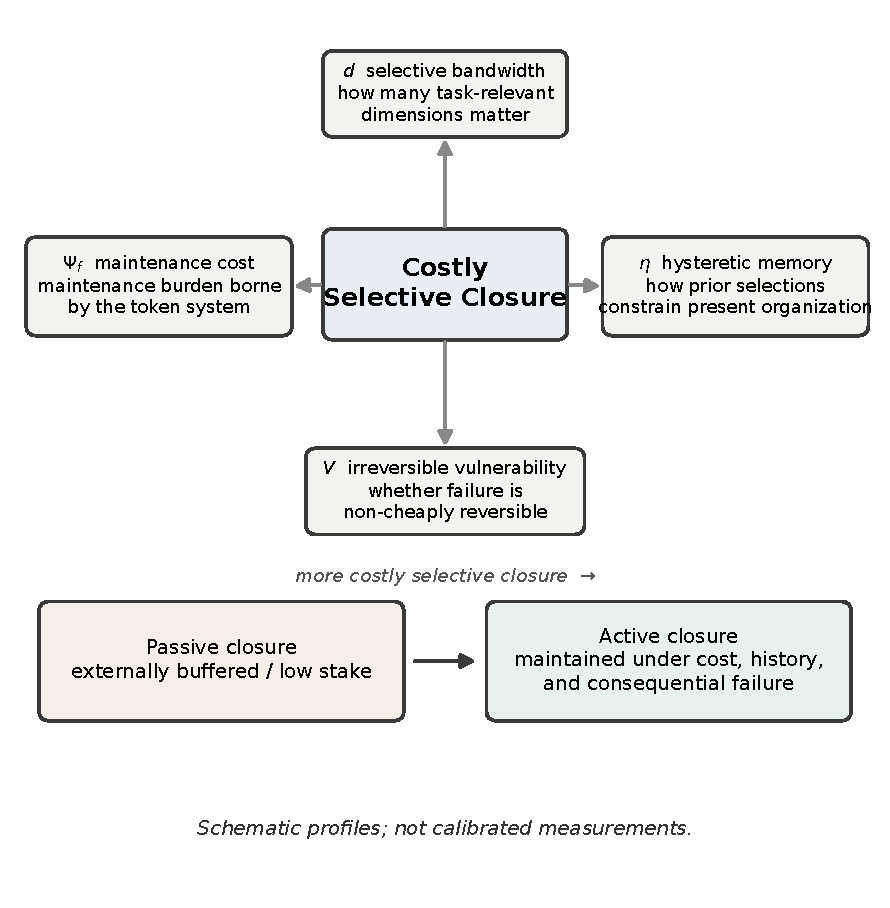
\includegraphics[width=0.9\linewidth,height=\textheight,keepaspectratio,alt={(Schematic.) The four dimensions of costly selective closure --- selective bandwidth d, maintenance cost \textbackslash Psi\_f, hysteretic memory \textbackslash eta, and irreversible vulnerability V --- shown as axes of a qualitative profile. The sketch is illustrative only: axis positions are ordinal placements for comparison, not calibrated measurements, and the figure should not be read as a precise radar chart.}]{figure1_framework.pdf}
\caption{\emph{(Schematic.)} The four dimensions of costly selective closure --- selective bandwidth \(d\), maintenance cost \(\Psi_f\), hysteretic memory \(\eta\), and irreversible vulnerability \(V\) --- shown as axes of a qualitative profile. The sketch is illustrative only: axis positions are ordinal placements for comparison, not calibrated measurements, and the figure should not be read as a precise radar chart.}
\end{figure}

\subsubsection{3.3 Passive and Active Closure}\label{passive-and-active-closure}

The framework distinguishes two broad regimes.

\textbf{Passive closure} describes systems that appear organized but whose organization is heavily buffered by external design, reset, or negligible consequence. They may be elegant, adaptive, and even behaviorally rich, yet they do not bear much of the burden of their own continued organization.

\textbf{Active closure} describes systems that must continuously pay to maintain their selected state, carry prior regulation forward, and risk genuine degradation if they fail.

This distinction matters because many debates about artificial life conflate the two. A system may display convincing local closure while remaining weakly life-like overall because its cost, memory, or vulnerability are shallow. The question is not whether closure exists at all, but whether it is passive or active.

\subsubsection{3.4 Status of the Formalization}\label{status-of-the-formalization}

The formalism above should be read as a qualitative-to-semi-quantitative comparison framework, not as a closed dynamical theory. The update equation is schematic: it states that current organization depends on present selection and retained history, but it does not assume that \(\hat{G}_\theta\) is linear, deterministic, or defined over a Euclidean state space. When state spaces are non-Euclidean, the weighted update should be understood as shorthand for any compatible local representation or state-update rule that preserves the same conceptual roles.

Likewise, the effective-rank definition of \(d\) is the principal definition, whereas \(d_{\mathrm{cog}}\) is an operational proxy intended for comparative work across substrates. The latter does not replace the former; it offers a practical route for approximate estimation when the full operator spectrum is not available. Finally, \(q\), \(P_{\mathrm{sel}}\), and \(N\) in the viability inequality should be treated as task-specific observables rather than already-standardized measurements. Difficult cases remain: systems with mirrored state, elastic cloud persistence, or dynamically shifting boundaries may only admit scenario-dependent estimates for \(\Psi_f\) and \(V\). The present framework is therefore best understood as a disciplined heuristic grammar for comparison and experiment design, not yet as a directly computable model.

\subsection{4. Canonical Cases}\label{canonical-cases}

Table~\ref{tab:canonical-cases} summarizes the framework's verdict on several familiar cases. The entries should be read as order-of-magnitude heuristic placements rather than measured quantities. At present the table is best understood as an ordinal scaffold for comparison: its value is to localize disagreement to one or more dimensions, not yet to report a calibrated ratio-scale measurement.

\begin{table*}[t]
\centering
\caption{Comparative heuristic profiles of canonical cases.}\label{tab:canonical-cases}
\begin{tabular}{@{}
  >{\raggedright\arraybackslash}p{(\linewidth - 10\tabcolsep) * \real{0.1667}}
  >{\raggedright\arraybackslash}p{(\linewidth - 10\tabcolsep) * \real{0.1667}}
  >{\raggedright\arraybackslash}p{(\linewidth - 10\tabcolsep) * \real{0.1667}}
  >{\raggedright\arraybackslash}p{(\linewidth - 10\tabcolsep) * \real{0.1667}}
  >{\raggedright\arraybackslash}p{(\linewidth - 10\tabcolsep) * \real{0.1667}}
  >{\raggedright\arraybackslash}p{(\linewidth - 10\tabcolsep) * \real{0.1667}}@{}}
\toprule
\begin{minipage}[b]{\linewidth}\raggedright
System
\end{minipage} & \begin{minipage}[b]{\linewidth}\raggedright
\(d\)
\end{minipage} & \begin{minipage}[b]{\linewidth}\raggedright
\(\Psi_f\)
\end{minipage} & \begin{minipage}[b]{\linewidth}\raggedright
\(\eta\)
\end{minipage} & \begin{minipage}[b]{\linewidth}\raggedright
\(V\)
\end{minipage} & \begin{minipage}[b]{\linewidth}\raggedright
Verdict
\end{minipage} \\
\midrule
Crystal & 0 & None & None & None & Stable but not life-like \\
Conway's Game of Life pattern & \textasciitilde0 & None & Very low & None & Organized update, not active closure \\
Lenia morphology & \textasciitilde1-3 & Low/emergent & Low & Low & Weakly life-like \\
Autopoietic/evolved embodied agent & \textasciitilde5-20 & Positive & Positive & Positive & Moderately life-like \\
Resettable RL agent & \textasciitilde2-20 & Often externally buffered & Positive & Weak & Behaviorally rich but shallow in stake \\
Biological organism & \textasciitilde{}\(10^{2}\text{--}10^{4}\) & Positive & Positive & Strong & Strong active closure \\
\bottomrule
\end{tabular}
\end{table*}

\subsubsection{4.1 Conway's Game of Life}\label{conways-game-of-life}

Game of Life (Gardner, 1970), heir to von Neumann's self-reproducing automata (von Neumann, 1966), remains a foundational example because it demonstrates how surprising pattern formation can emerge from simple rules. Yet, under the present framework, it ranks low in life-likeness. Patterns localize and persist, but they do not bear non-trivial cost, retain history in a robust sense, or face consequential failure. The most sustained attempt to read a Game of Life pattern as an autopoietic individual (Beer, 2004) is instructive here: it recovers organizational closure and structural coupling, but the pattern's self-production remains a feature of the observer's descriptive stance rather than a cost borne by the token to remain what it is. The system updates according to fixed rules; it does not actively maintain a selected mode of existence under burden.

\subsubsection{4.2 Lenia}\label{lenia}

Lenia (Chan, 2019) is more interesting because it produces morphologies with clear behavioral coherence. Patterns move, stabilize, regenerate, and sometimes appear to ``seek'' conditions that preserve form. This gives Lenia stronger localization and a weak analogue of maintenance cost: the pattern must continually sustain itself against dispersion. The placement \(d \sim 1\text{--}3\) reflects the fact that Lenia's update kernel and stable morphologies usually organize variation around a small number of dominant spatial modes, such as translation, oscillation, and orientation, rather than a broad set of independently weighted environmental variables. Even so, its hysteresis is limited and its vulnerability is shallow compared with embodied agents. It is therefore best described as weakly life-like.

\subsubsection{4.3 Autopoietic Agents}\label{autopoietic-agents}

Embodied autopoietic or evolved agents in the dynamical-systems and enactive tradition (Beer, 1995; Di Paolo, 2005) score higher. They regulate sensorimotor coupling, maintain a boundary, and can fail in ways that matter for continued performance. Their current activity is constrained by prior adaptation, which gives them a meaningful \(\eta\), and their continued organization requires ongoing work, which gives them positive \(\Psi_f\). The rough placement \(d \sim 5\text{--}20\) should be read as assuming a system that must jointly track several partially independent variables, for example resource gradient, orientation, collision risk, boundary integrity, and a small number of partner or obstacle states, without yet exhibiting the broader temporal and social concern-spaces of complex organisms. Such systems are among the clearest artificial demonstrations of active closure currently available.

\subsubsection{4.4 Resettable Digital Agents}\label{resettable-digital-agents}

Many contemporary digital agents complicate the picture. Reinforcement-learning systems can exhibit substantial behavioral flexibility and therefore non-trivial \(d\), but the scale of \(d\) depends strongly on architecture and task. The deliberately minimal cooperative experiment discussed below yields \(d_{\mathrm{eff}}\) values below 2, whereas richer agents with broader sensory, temporal, or social coupling could plausibly extend into the teens. They may also carry substantial training history and internal state, giving them non-trivial \(\eta\). But if their organization is extensively buffered by cheap reset, abundant copying, and negligible irreversible loss, then \(V\) remains weak and \(\Psi_f\) is not borne by the agent in a robust sense. They are therefore best treated as partial life-likeness: high behavioral sophistication under shallow stake conditions. The same point applies, even more strongly, to contemporary large language models.

\subsubsection{4.5 A Controlled Experiment: Isolating the Vulnerability Dimension}\label{a-controlled-experiment-isolating-the-vulnerability-dimension}

To test whether token-level irreversibility does causal work rather than merely labeling systems after the fact, we run a controlled two-agent experiment in a PettingZoo-style cooperative survival environment (Terry et al., 2021). Two \emph{independent} policies are trained with REINFORCE (Williams, 1992), each a two-layer network over 12 observation features with three actions (\emph{cooperate}, \emph{solo}, \emph{rest}). The immediate reward is ordered as a Prisoner's Dilemma (temptation 1.4 \textgreater{} mutual cooperation 1.0 \textgreater{} mutual defection 0.6 \textgreater{} sucker 0.0), so unilateral defection is always tempting; but the energy economy ties survival to coordination, since only mutual cooperation yields net-positive energy while mutual defection slowly starves both agents. Each agent is trained with a mutual-cooperation bonus for 1000 episodes, after which the bonus is withdrawn and 300 online-adaptation episodes follow. The \textbf{real-stake} and \textbf{resettable} regimes share an identical reward function and differ in one variable only: in the real-stake regime, energy depletion terminates the token run, whereas in the resettable regime the depleted agent is restored to full energy and the run continues. A third, auxiliary \textbf{simulated-stake} regime remains resettable but adds a mortality cue to the observation and an additional represented-danger reward penalty. The clean causal comparison therefore concerns real stake versus cheap reset; token-level irreversibility is the sole variable separating them. The simulated-stake condition instead tests whether representing danger without removing restoration is sufficient to reproduce the real-stake effect. The design deliberately avoids the failure of an earlier pilot in which cooperation was weakly reward-dominant and death almost never occurred, so that the real and resettable regimes were indistinguishable.

\begin{figure}
\centering
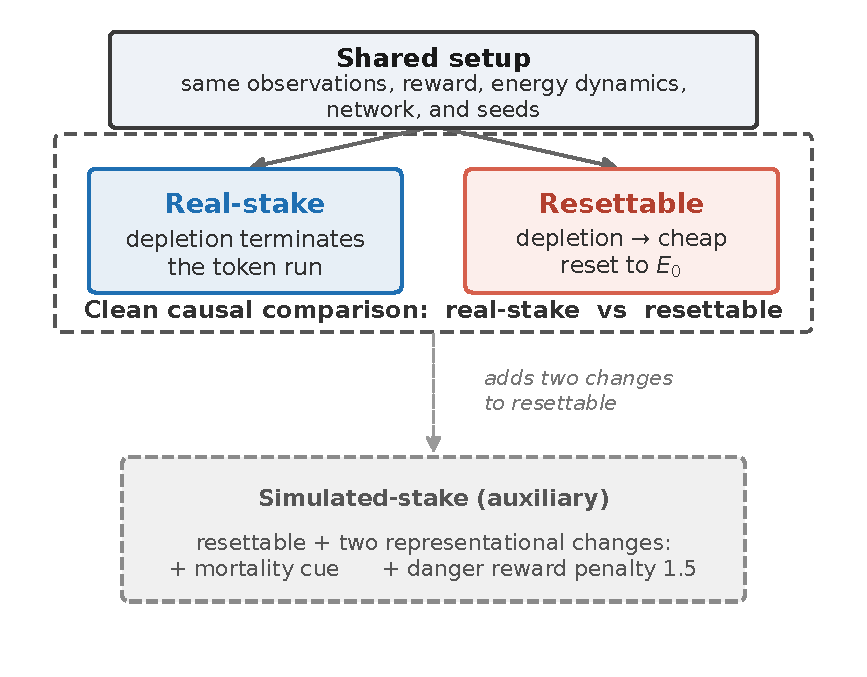
\includegraphics[width=0.9\linewidth,height=\textheight,keepaspectratio,alt={Experimental design and lifecycle regimes. Real-stake and resettable agents share matched rewards and differ only in terminate-versus-reset on depletion. The auxiliary simulated-stake condition remains resettable while adding a mortality observation cue and an extra represented-danger reward penalty.}]{figure2_design.pdf}
\caption{Experimental design and lifecycle regimes. Real-stake and resettable agents share matched rewards and differ only in terminate-versus-reset on depletion. The auxiliary simulated-stake condition remains resettable while adding a mortality observation cue and an extra represented-danger reward penalty.}
\end{figure}

In the compact bookkeeping map, the designed environment and its action-contingent futures supply the local possibility space, the currently occupied observation-action regime forms the maintained state, and the trained policy weights plus recent-history observation channels provide the simplest form of retained constraint. Here \(d\) is estimated from the effective rank of the Jacobian of the action logits with respect to the 12 observation features across held-out states, using the concatenated Jacobian and

\[
d_{eff} = \frac{\left(\sum_i \lambda_i\right)^2}{\sum_i \lambda_i^2}.
\]

Across 30 seeds this yields mean \(d_{\mathrm{eff}}\) values near 1.5 to 1.8 in all three regimes, with the low absolute values reflecting the deliberately narrow concern-space of the toy architecture. Because \(d\) is comparable across the regimes, it is treated here as a descriptive read rather than the tested variable; the manipulation targets \(V\).

In this experiment, \(\eta\) is modest rather than large, because historical carry-over enters only through short-horizon observation memory and learned policy weights, not through a recurrent latent state. \(\Psi_f\) differs mainly in who bears the maintenance burden: the resettable and simulated regimes are externally buffered, whereas in the real-stake regime loss ends the token run. \(V\) is therefore weakest in the resettable condition, strongest in the real-stake condition, and intermediate in the simulated condition, for which danger is represented but restoration remains architecturally available.

After the bonus is withdrawn, mutual cooperation is sustained only under real stake. Across 30 seeds, post-withdrawal mutual cooperation averages 0.55 in the real-stake regime against 0.04 (resettable) and 0.07 (simulated). Because the real and resettable regimes share seeds, the primary test is a two-sided paired sign-flip permutation test on the per-seed real−resettable differences (\(p < 0.0001\), 20,000 resamples); a pooled unpaired permutation test agrees (\(p < 0.0001\)). The divergence is already visible during training: resettable agents fail to commit to cooperation even while the bonus is active, because cheap restoration lets them collect the defection payoff and shrug off starvation, dying and resetting several times per episode. Under matched reward, then, the mere availability of a cheap restore is enough to prevent costly cooperation from ever stabilizing.

Three robustness checks guard against the obvious objections. First, when the explicit death penalty is removed entirely, so that the only consequence of depletion is that the return stream ends, the separation is essentially unchanged (0.50 versus 0.05; because these regimes also share seeds, a paired sign-flip permutation test gives \(p < 0.0001\), and the pooled unpaired test agrees); the effect is therefore driven by return-truncation itself, not by a hand-tuned penalty. Second, generalizing the binary contrast to a graded maximum number of lives produces a monotone dose-response: post-withdrawal cooperation falls from 0.54 with a single life, through 0.16 with two lives, to 0.03 with four or more (tie-aware Spearman -0.44, blocked-by-seed permutation \(p < 0.0001\), between the life budget and cooperation). The unbounded result equals the four-life result, so the collapse is not an artifact of an unbounded life budget. Third, across a payoff sweep spanning three temptation values and two starvation rates, real exceeds resettable in every one of the six cells.

\begin{figure*}
\centering
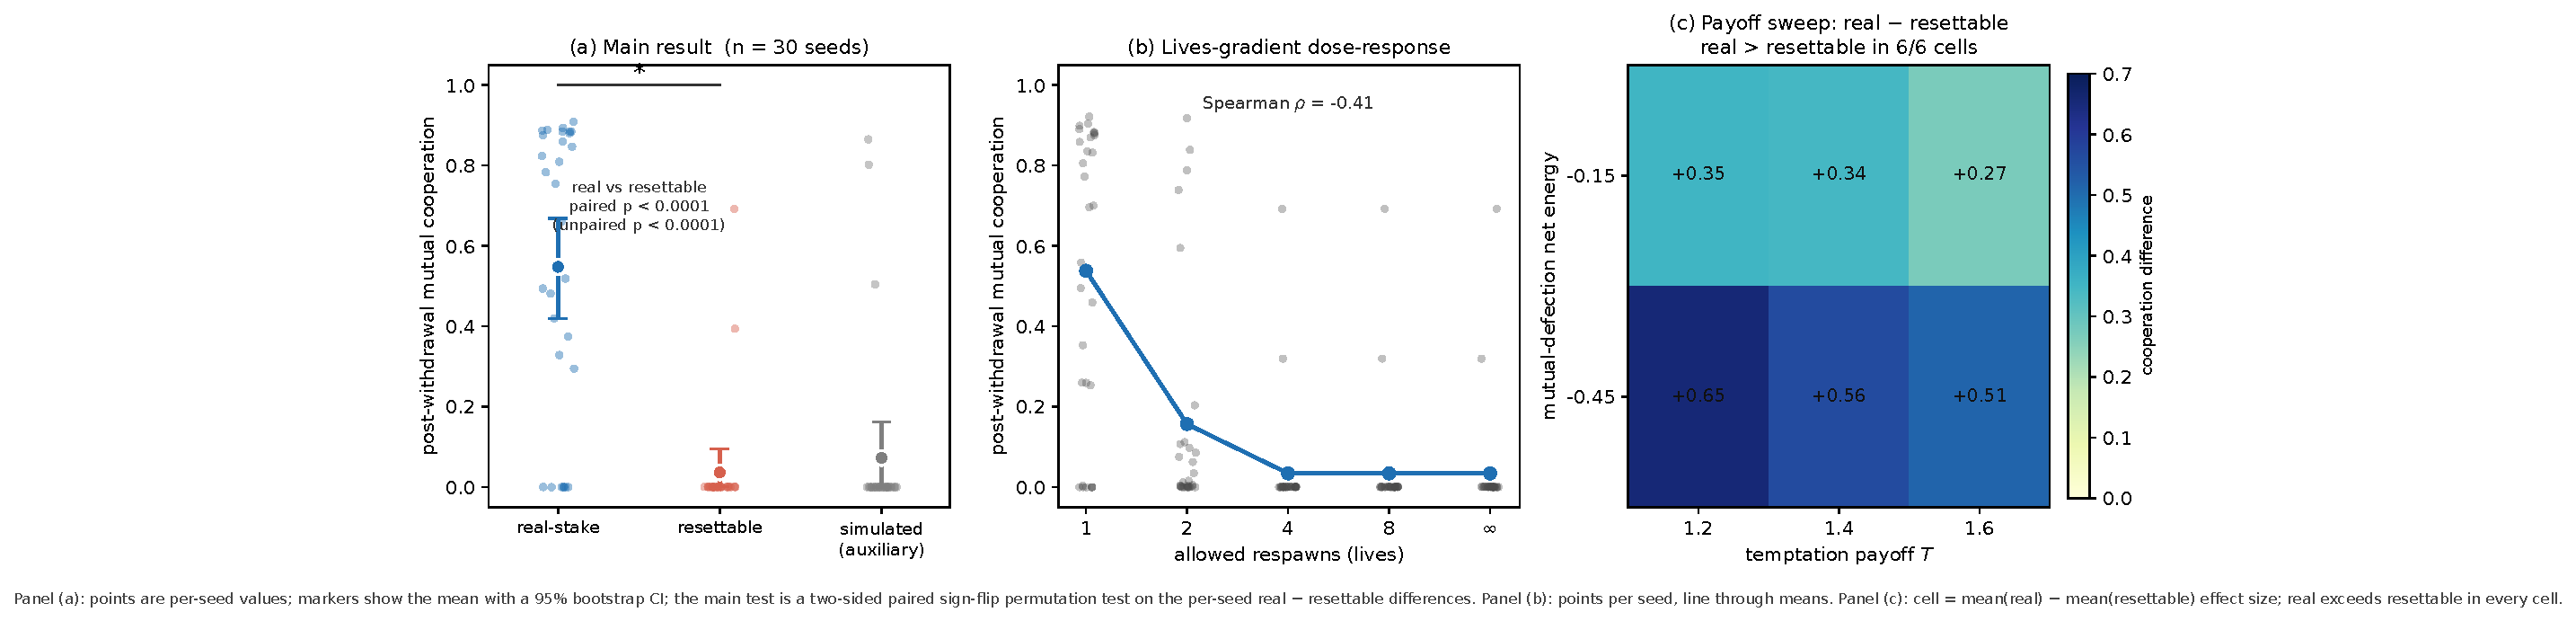
\includegraphics[width=0.9\linewidth,height=\textheight,keepaspectratio,alt={Main result and robustness, generated from the committed result files. (a) Post-withdrawal mutual cooperation by regime (real 0.55, resettable 0.04, simulated 0.07; n = 30 seeds); points are per-seed values and markers show the mean with a 95\% bootstrap confidence interval; the main test is a two-sided paired sign-flip permutation test (real vs resettable, p \textless{} 0.0001; a pooled unpaired test agrees). (b) Lives-gradient dose-response: post-withdrawal cooperation as a function of the maximum number of lives (1, 2, 4, 8, ∞), with the monotone decline from \textasciitilde0.54 at one life to \textasciitilde0.03 at four or more (tie-aware Spearman ρ = −0.44, blocked-by-seed permutation p \textless{} 0.0001). (c) Payoff sweep: the real − resettable cooperation difference across three temptation values and two starvation settings, positive (real \textgreater{} resettable) in all six cells.}]{figure3_results.pdf}
\caption{Main result and robustness, generated from the committed result files. (a) Post-withdrawal mutual cooperation by regime (real 0.55, resettable 0.04, simulated 0.07; n = 30 seeds); points are per-seed values and markers show the mean with a 95\% bootstrap confidence interval; the main test is a two-sided paired sign-flip permutation test (real vs resettable, p \textless{} 0.0001; a pooled unpaired test agrees). (b) Lives-gradient dose-response: post-withdrawal cooperation as a function of the maximum number of lives (1, 2, 4, 8, ∞), with the monotone decline from \textasciitilde0.54 at one life to \textasciitilde0.03 at four or more (tie-aware Spearman ρ = −0.44, blocked-by-seed permutation p \textless{} 0.0001). (c) Payoff sweep: the real − resettable cooperation difference across three temptation values and two starvation settings, positive (real \textgreater{} resettable) in all six cells.}
\end{figure*}

A residual concern is that the rollout cooperation measure is affected by unequal episode lengths: real-stake episodes can terminate early, whereas resettable episodes continue to the fixed horizon, and cooperation is computed only over steps in which both agents remain alive. We therefore ran a frozen-policy common-state probe. Policies from every regime and seed were scored on the same global bank of 2,292 paired observations, built from mortality-free states lying in the empirical common support of independently generated real-stake and resettable rollouts (with bank-generation seeds disjoint from the evaluated policies). On identical states at the end of withdrawal, expected mutual cooperation was 0.485 under real stake and 0.030 under cheap reset, a paired difference of 0.454 (95\% bootstrap CI {[}0.346, 0.557{]}; paired sign-flip permutation \(p < 0.0001\)); a comparably large separation was already present at the end of training (0.546 versus 0.043). The rollout difference therefore cannot be explained solely by unequal trajectory lengths or by restricting the cooperation denominator to surviving steps. The probe does not remove training-time differences in return structure and state occupancy, which are the mechanisms through which the terminate-versus-reset intervention shapes the learned policies; the full procedure is given in the Appendix.

\begin{figure*}
\centering
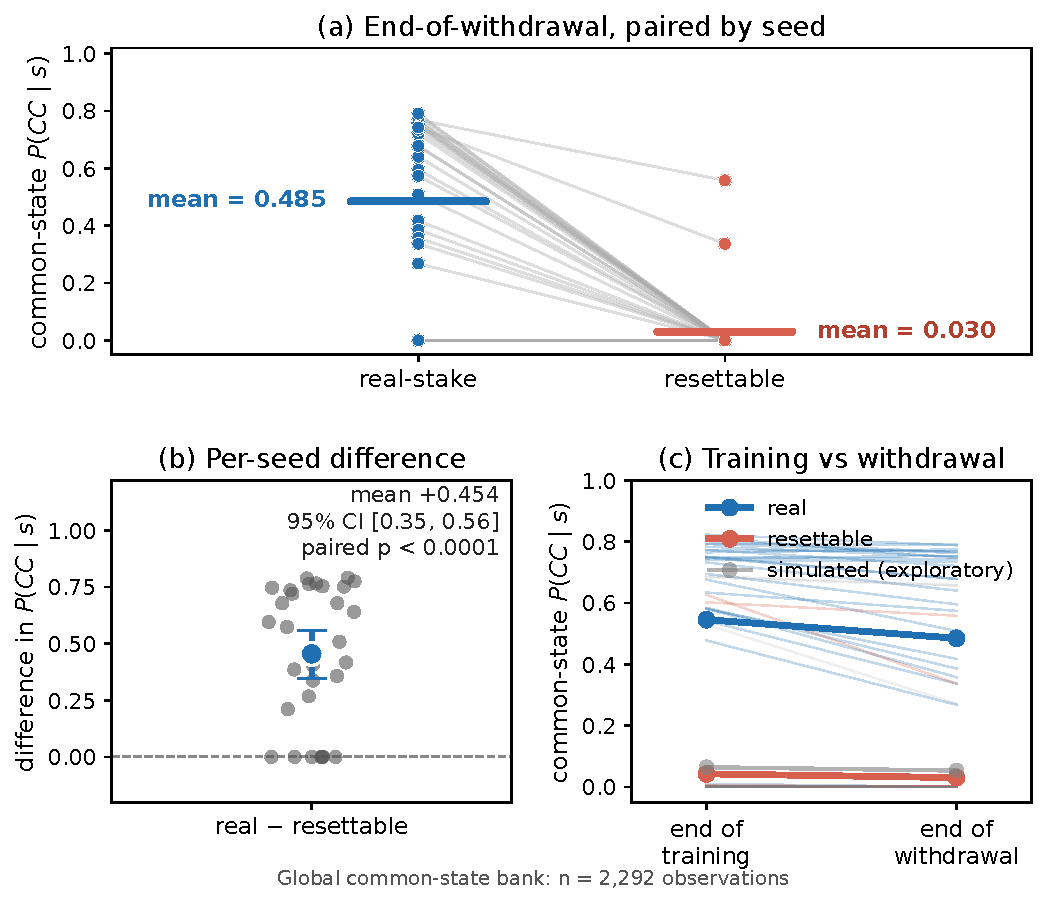
\includegraphics[width=0.9\linewidth,height=\textheight,keepaspectratio,alt={Common-state frozen-policy probe, generated from the committed probe result file. Every regime's frozen policies are scored on one global bank of 2,292 mortality-free paired observations in the real--resettable common support. (a) End-of-withdrawal expected mutual cooperation P(CC \textbar{} s) per seed, real versus resettable, with paired connecting lines. (b) Per-seed real − resettable differences with the mean and 95\% bootstrap CI. (c) End-of-training versus end-of-withdrawal per regime. Simulated-stake is shown only as a faded secondary reference. Points are per-seed values; no density smoothing is used.}]{figure4_common_state_probe.pdf}
\caption{Common-state frozen-policy probe, generated from the committed probe result file. Every regime's frozen policies are scored on one global bank of 2,292 mortality-free paired observations in the real--resettable common support. (a) End-of-withdrawal expected mutual cooperation P(CC \textbar{} s) per seed, real versus resettable, with paired connecting lines. (b) Per-seed real − resettable differences with the mean and 95\% bootstrap CI. (c) End-of-training versus end-of-withdrawal per regime. Simulated-stake is shown only as a faded secondary reference. Points are per-seed values; no density smoothing is used.}
\end{figure*}

Taken together, these results provide controlled evidence that token-level irreversibility can act as a causal control variable under matched reward landscapes. The experiment should still be read for exactly what it establishes and no more. Within this deliberately survival-coupled testbed, the terminate-versus-reset intervention --- used here as an operationalization of episode-token vulnerability --- causally changes the learned policies: cheap restoration strongly suppresses the costly cooperative behavior tested here. It does not validate the four-dimensional framework jointly, since \(d\) and \(\eta\) are held roughly fixed and are descriptive here; and the environment is deliberately a testbed in which survival depends on the costly behavior, so the finding is the magnitude of the effect, its dose-response, and its disappearance under a cheap restore, not a claim that irreversibility matters in every environment. The mechanism is close to an elementary property of reinforcement learning: terminating an agent's return stream makes a reward-maximizer avoid the terminating event. That is consistent with, rather than embarrassing to, the framework, because it is precisely why an episode-terminating reinforcement learner carries a nonzero but shallow \(V\) and sits at the ``weakly life-like'' placement of Table~\ref{tab:canonical-cases}. Three organizational levels should be kept distinct. Termination acts at the \emph{episode-token} level: the depleted agent's current run ends. Learning and historical accumulation occur at the \emph{controller-lineage} level, where the policy weights persist across episodes and keep updating; a token's death does not delete them. Selection pressure is applied by the \emph{training process} over many episodes. The manipulation therefore controls whether each within-episode failure is terminal; it does not construct a self-contained digital organism whose controller is physically destroyed on death. What the experiment tests is how episode-token termination shapes the across-episode learning pressure, and the common-state probe indicates that, in this environment, the effect appears as a difference in the learned policies rather than only in the rollout measurement window. Full experimental details are given in the Appendix, and an anonymized reproduction package (code, fixed result files, and figure scripts) is provided as supplementary material.

\subsubsection{4.6 Biological Organisms}\label{biological-organisms}

Biological organisms remain the strongest paradigm case because all four dimensions are tightly coupled. Their selective bandwidth is non-trivial, their maintenance cost is ongoing, their history is sedimented into morphology and regulation, and failure can irreversibly damage or destroy the organized whole. The coarse placement \(d \sim 10^{2}\text{--}10^{4}\) is deliberately taxonomically heterogeneous; it is included only to register expected scale separation once spatial, interoceptive, temporal, and social concern dimensions are jointly counted, not as a calibrated claim about any single species. The framework therefore preserves the intuition that ordinary living systems are not merely more complex than passive artifacts; they are organized under a more demanding regime of maintenance and consequence.

\subsection{5. Borderline Cases: Discriminating Profiles}\label{borderline-cases-discriminating-profiles}

A comparative heuristic earns its keep on hard cases. The most cited challenges to any account of life --- viruses and prions --- are usually posed as yes/no questions and answered by fiat. The present framework declines the yes/no framing. Because life-likeness here is a four-dimensional profile rather than a threshold, a borderline system is not classified but \emph{placed}, and the placement makes discriminating, in-principle checkable claims about which dimension carries the case. Table~\ref{tab:borderline-cases} profiles four systems that a one-dimensional criterion tends to collapse together.

\begin{table*}[t]
\centering
\caption{Discriminating profiles of borderline cases at the stated organizational level.}\label{tab:borderline-cases}
\begin{tabular}{@{}
  >{\raggedright\arraybackslash}p{(\linewidth - 10\tabcolsep) * \real{0.1667}}
  >{\raggedright\arraybackslash}p{(\linewidth - 10\tabcolsep) * \real{0.1667}}
  >{\raggedright\arraybackslash}p{(\linewidth - 10\tabcolsep) * \real{0.1667}}
  >{\raggedright\arraybackslash}p{(\linewidth - 10\tabcolsep) * \real{0.1667}}
  >{\raggedright\arraybackslash}p{(\linewidth - 10\tabcolsep) * \real{0.1667}}
  >{\raggedright\arraybackslash}p{(\linewidth - 10\tabcolsep) * \real{0.1667}}@{}}
\toprule
\begin{minipage}[b]{\linewidth}\raggedright
System (level)
\end{minipage} & \begin{minipage}[b]{\linewidth}\raggedright
\(d\)
\end{minipage} & \begin{minipage}[b]{\linewidth}\raggedright
\(\Psi_f\) (token)
\end{minipage} & \begin{minipage}[b]{\linewidth}\raggedright
\(\eta\)
\end{minipage} & \begin{minipage}[b]{\linewidth}\raggedright
\(V\) (token)
\end{minipage} & \begin{minipage}[b]{\linewidth}\raggedright
Reading
\end{minipage} \\
\midrule
Prion & \textasciitilde0 & \textasciitilde0 & Moderate (structural template) & \textasciitilde0 & Replicates and inherits, pays nothing \\
Free virion & Very low & \textasciitilde0 & Genomic & Low (structural) & Organized structure, latent instructions \\
Virus, replicating (virion token) & Low & \textasciitilde0 (host-borne) & Genomic & Low & Maintenance cost externalized to host \\
Dormant spore & \textasciitilde0 & \textasciitilde0 & Maximal & Low (robust) & \(\eta\) retained, other dimensions collapsed \\
Germinated organism & Positive & Positive & Positive & Positive & Active closure restored \\
Resettable digital agent & Moderate-high & Externalized & Positive & \textasciitilde0 & High bandwidth, shallow stake \\
\bottomrule
\end{tabular}
\end{table*}

\emph{Note.} The token evaluated in each row is the individual unit named; for the virus it is the virion. The coupled virus-host process may receive a different profile, since vulnerability is level-indexed (see ``Vulnerability is level-indexed'' below).

\textbf{Prion.} A prion propagates by templating its own misfolded conformation (Prusiner, 1998). It reproduces and it inherits --- a faithful information carrier --- yet it pays essentially no maintenance cost (\(\Psi_f \sim 0\); the misfolding is thermodynamically favored, not sustained against decay) and couples to no world beyond its template (\(d \sim 0\)). The framework therefore places the prion \emph{below} the virus in life-likeness, driven entirely by the collapse of \(\Psi_f\) and \(d\). This is a discriminating prediction: a criterion keyed on replication or heritable information --- the replicator-paradigm view on which the aliveness question is settled by information transmission (Koonin and Starokadomskyy, 2016) --- would rank the prion at least as high as any other faithful replicator, whereas costly selective closure places it near the floor. The prion is exactly the case on which the information-centric and cost-centric readings of life come apart.

\textbf{Virus.} Whether viruses count as alive is the classic borderline dispute (Forterre, 2010). A free virion is an organized structure carrying latent instructions: low \(d\), \(\Psi_f \sim 0\), phylogenetic history in the genome (\(\eta\)), and a token vulnerability that is structural fragility rather than failure of self-maintenance. During replication the picture seems to change, but the maintenance cost is borne by the \emph{host}, not the virion. The framework's discriminating claim is that the virus's token \(\Psi_f\) stays near zero even mid-replication, because the burden is externalized --- the same pattern that flags resettable digital agents. It predicts that partitioning the energetics of infection between virion and host assigns the active maintenance cost to the host cell, and locates whatever life-likeness is present in the coupled virus-host system rather than in the virion alone.

\textbf{Dormant spores and seed banks.} A dormant spore is metabolically inert (Lennon and Jones, 2011): \(d\) and \(\Psi_f\) fall to near zero and its token vulnerability is low, since dormancy is precisely a robustness adaptation, while \(\eta\) is maximal --- the spore is almost pure sedimented structure, carrying the whole organization forward. The framework predicts that life-likeness is \emph{phase-dependent} rather than a fixed property of a genome: across a sporulation-germination cycle the same lineage traces a large swing in \(d\), \(\Psi_f\), and \(V\) while \(\eta\) stays nearly constant, and only germination restores active closure. This is where autopoiesis and active inference strain --- a dormant spore performs neither, yet we resist calling it dead --- and where the profile view answers without strain: the spore is momentarily low on three dimensions and maximal on the fourth, and it is the retained \(\eta\) that bridges back to reactivation.

\textbf{Resettable digital agents.} Placed here for contrast, contemporary digital agents occupy a corner no biological borderline case reaches: potentially high \(d\) with near-zero token \(V\), their \(\Psi_f\) externalized to servers and their history retained in weights. The framework predicts that this high-bandwidth, low-vulnerability profile is behaviorally rich but shallow in stake, and that its apparent commitments collapse when the buffering is removed --- the effect shown in Section 4.5. The borderline biological cases show that the same profile logic that reads a digital agent also reads a virion, a prion, and a spore, on one shared set of axes.

\textbf{Vulnerability is level-indexed.} These placements are well-formed only once a level of organization is fixed, because \(V\) is level-indexed, echoing the long-recognized hierarchy of units of selection and Darwinian individuality (Lewontin, 1970; Godfrey-Smith, 2009): the same physical system carries different vulnerability as a single virion, an infected cell, a quasispecies, or a lineage; as a single spore or a seed bank; as one agent instance or a swarm of checkpoints. Failing to fix the level manufactures spurious disputes. The units-of-selection objection --- that a population supplies cheap backup, so the individual organism does not matter (Section 2) --- is precisely the observation that lineage-level \(V\) can be low while token-level \(V\) is high. The framework does not legislate which level is privileged. It requires that a life-likeness claim declare its level, and it suggests that the theoretically interesting systems are those whose token-level and lineage-level vulnerability diverge: suicidal altruists paying high token \(V\) in service of a buffered lineage, clonal colonies, seed banks, and resettable agent swarms. On this reading, altruistic self-sacrifice is not a counterexample to the heuristic but a case it anticipates --- high token vulnerability deployed under low lineage vulnerability.

None of this delivers a definition of life, and none of it is offered as proof that any of these systems is or is not alive. The claims are comparative and, in principle, checkable: they say where a system falls on four axes, how its profile shifts across phase and level, and which dimension carries a given disagreement. What distinguishes costly selective closure from a single-axis criterion is just this --- it converts ``is X alive?'' into ``what is X's profile, at which level?'', and it makes the borderline cases disagree with rival criteria at nameable points.

\subsection{6. Artificial Life as Experimental Philosophy}\label{artificial-life-as-experimental-philosophy}

The value of the framework lies not only in classification but in construction. If life-likeness depends on the coupled presence of bandwidth, cost, memory, and vulnerability, then artificial life can manipulate each of these dimensions directly. This is what philosophy looks like when it has to be built.

Three design lessons follow immediately.

First, \textbf{increasing bandwidth alone is not enough}. A system can become better at tracking and exploiting multiple dimensions while remaining weakly life-like if its costs and consequences are buffered. This is one reason why high-capability digital systems can appear agentic without becoming strong candidates for life-likeness.

Second, \textbf{cost without bandwidth is not enough}. A system may consume energy or degrade physically while remaining behaviorally trivial. Mere expenditure does not create life-like organization; the expenditure must support selective closure across a non-trivial space.

Third, \textbf{memory without vulnerability is not enough}. Rich retained structure can yield impressive persistence and adaptation, but if regulatory failure can always be undone at negligible cost, the system's commitments remain shallow.

The clearest experimental consequence is a design built around one matched causal contrast and one auxiliary condition.

\begin{enumerate}
\def\labelenumi{\arabic{enumi}.}
\tightlist
\item
  \textbf{Real-stake}: depletion terminates the token run.
\item
  \textbf{Resettable}: same observations, rewards, and resource dynamics as real-stake, but depletion triggers cheap restoration.
\item
  \textbf{Simulated-stake}: remains resettable while receiving mortality cues and/or additional danger-related penalties.
\end{enumerate}

A concrete testbed would be a PettingZoo-style gridworld with scarce food patches, pairwise carrying or sharing actions, energy depletion, and scheduled perturbation events. In the real-stake condition, depletion terminates the token run. In the resettable condition, depletion reinstantiates the same policy with restored energy. In the simulated-stake condition, reset remains available but the agent receives mortality cues and additional danger-related penalties. For the clean causal comparison, reward functions, observation spaces, and background resource density should remain matched between the real-stake and resettable conditions, so that the only manipulated variable is terminate-versus-reset. The simulated-stake condition is auxiliary: it may add explicit mortality cues or danger-related penalties in order to test whether represented risk can substitute for non-cheaply reversible failure.

The prediction is not merely that the first class will perform differently. It is that only the first class should stably preserve certain long-horizon properties after reward withdrawal or perturbation: costly cooperation, durable commitment, and meaningful post-shock recovery. Resettable agents may learn these behaviors, but their persistence should be shallower; simulated-stake agents may initially resemble real-stake agents, yet their commitments should degrade once experience reveals that apparent risk is externally buffered. The controlled experiment in Section 4.5 realizes this design. In the clean matched comparison, real-stake agents stabilize costly cooperation whereas resettable agents collapse to defection. The auxiliary simulated-stake condition also collapses despite receiving an explicit mortality cue and additional danger-related penalty, suggesting that representing danger is not sufficient when cheap restoration remains available. The separation scales monotonically with the degree of irreversibility. This is evidence for the framework's core claim in one carefully built environment. It is not yet evidence that the same separation survives across substrates, richer state spaces, or genuinely open-ended settings, which remains the natural next test.

This also suggests a link to open-ended evolution (OEE). On the present view, open-ended evolutionary dynamics can be interpreted as costly selective closure operating across lineage time, where selective commitments are not only maintained within agents but accumulated, revised, and amplified across adaptive transitions. Recent OEE work has increasingly emphasized behavioral hallmarks, domain-specific measures, and the difficulty of obtaining a single universal metric, which is congenial to the present framework's dimensional approach (Adams et al., 2017; Borg et al., 2024; Channon et al., 2024).

This does not prove that any given artificial agent is alive. It does something more useful: it converts ``what is life-like?'' into a buildable discrimination problem. The philosophical claim is therefore experimentally exposed. If cost, memory, and vulnerability can be stripped away without changing the persistence of life-like behavior, then the framework is wrong or incomplete. If they cannot, then costly selective closure marks a real boundary in the design space of artificial life. The present contribution remains primarily heuristic and programmatic, but it now rests on a controlled experiment rather than only an experimental sketch. A frozen-policy probe on matched states indicates that the central real-versus-resettable contrast reflects a difference in the learned policies rather than a measurement-window artifact, without extending the broader life-likeness claim.

\subsection{7. Conclusion}\label{conclusion}

Artificial life needs comparative tools that are broad enough to compare different substrates and sharp enough to guide construction. This paper has argued that \textbf{costly selective closure} offers one such comparative heuristic. A system is more life-like not simply because it persists, reproduces, predicts, or behaves adaptively, but to the extent that it selectively maintains a world under non-trivial cost, historical carry-over, and consequential failure.

The framework does not offer a final essence of life, and it does not claim that there is a single bright line between the living and the non-living. Its aim is practical: it gives artificial life a compact, buildable set of dimensions that can be engineered, varied, and tested. In that sense it is close to Thompson's gradient view of life and mind, while remaining more pluralistic about which organizational forms may count as partial cases of life-likeness beyond standard autopoietic models (Thompson, 2007). It also sits naturally beside basal-cognition approaches that treat memory, valence, and adaptive problem solving as deeply distributed across living organization, while remaining focused here on life-likeness rather than consciousness per se (Lyon et al., 2021; Lyon and Cheng, 2023; Birch et al., 2020). Cross-substrate calibration remains open; assembly depth may provide one useful anchor for the complexity term in \(d_{\mathrm{cog}}\) (Sharma et al., 2023).

The central lesson is simple: stronger life-likeness requires stronger forms of paid commitment. To build a more life-like system, it is not enough to increase complexity, realism, or behavioral flexibility. Artificial systems must be built so that their organization matters because it must be maintained, carried forward, and can genuinely be lost.

\subsection{Data and Code Availability}\label{data-and-code-availability}

An anonymized reproduction package containing the experiment code, the fixed result files used in the paper, and the figure-generation scripts is provided as supplementary material. All quantitative content in Figure 3 is regenerated from the committed result files by the included figure script; no values are hand-entered. The clean causal comparison is real-stake versus resettable; the simulated-stake condition is auxiliary.

\section*{References}

Adams, A., Zenil, H., Davies, P. C. W., and Walker, S. I. (2017). Formal definitions of unbounded evolution and innovation reveal universal mechanisms for open-ended evolution in dynamical systems. \emph{Scientific Reports}, 7, 997.

Aguilera, M., Millidge, B., Tschantz, A., and Buckley, C. L. (2022). How particular is the physics of the free energy principle? \emph{Physics of Life Reviews}, 40, 24-50.

Aubin, J.-P. (1991). \emph{Viability Theory}. Birkhäuser.

Baltieri, M., and Suzuki, K. (2025). Mathematical approaches to the study of agents. \emph{Philosophical Transactions of the Royal Society B} (in press).

Beer, R. D. (1995). A dynamical systems perspective on agent-environment interaction. \emph{Artificial Intelligence}, 72(1-2), 173-215.

Beer, R. D. (2004). Autopoiesis and cognition in the Game of Life. \emph{Artificial Life}, 10(3), 309-326.

Birch, J., Ginsburg, S., and Jablonka, E. (2020). Unlimited Associative Learning and the origins of consciousness: a primer and some predictions. \emph{Biology \& Philosophy}, 35, 56.

Borg, J. M., Buskell, A., Kapitany, R., Powers, S. T., Reindl, E., and Tennie, C. (2024). Evolved open-endedness in cultural evolution: A new dimension in open-ended evolution research. \emph{Artificial Life}, 30(3), 417-438.

Chan, B. W.-C. (2019). Lenia: Biology of artificial life. \emph{Complex Systems}, 28(3), 251-286.

Channon, A., Bedau, M. A., Packard, N. H., and Taylor, T. (2024). Editorial introduction to the 2024 special issue on open-ended evolution. \emph{Artificial Life}, 30(3), 300-301.

Di Paolo, E. A. (2005). Autopoiesis, adaptivity, teleology, agency. \emph{Phenomenology and the Cognitive Sciences}, 4(4), 429-452.

Egbert, M. D., and Barandiaran, X. E. (2011). Quantifying normative behavior and precariousness in adaptive agency. In \emph{Advances in Artificial Life (ECAL 2011)}, 210-217.

Forterre, P. (2010). Defining life: the virus viewpoint. \emph{Origins of Life and Evolution of Biospheres}, 40(2), 151-160.

Froese, T., and Ziemke, T. (2009). Enactive artificial intelligence: Investigating the systemic organization of life and mind. \emph{Artificial Intelligence}, 173(3-4), 466-500.

Friston, K. J. (2013). Life as we know it. \emph{Journal of the Royal Society Interface}, 10(86), 20130475.

Gardner, M. (1970). Mathematical games: The fantastic combinations of John Conway's new solitaire game ``life''. \emph{Scientific American}, 223(4), 120-123.

Godfrey-Smith, P. (2009). \emph{Darwinian Populations and Natural Selection}. Oxford University Press.

Kirchhoff, M. D., Parr, T., Palacios, E., Friston, K. J., and Kiverstein, J. (2018). The Markov blankets of life: Autonomy, active inference and the free energy principle. \emph{Journal of the Royal Society Interface}, 15(138), 20170792.

Koonin, E. V., and Starokadomskyy, P. (2016). Are viruses alive? The replicator paradigm sheds decisive light on an old but misguided question. \emph{Studies in History and Philosophy of Biological and Biomedical Sciences}, 59, 125-134.

Lennon, J. T., and Jones, S. E. (2011). Microbial seed banks: the ecological and evolutionary implications of dormancy. \emph{Nature Reviews Microbiology}, 9(2), 119-130.

Lewontin, R. C. (1970). The units of selection. \emph{Annual Review of Ecology and Systematics}, 1, 1-18.

Lyon, P., Keijzer, F., Arendt, D., and Levin, M. (2021). Reframing cognition: getting down to biological basics. \emph{Philosophical Transactions of the Royal Society B}, 376, 20190750.

Lyon, P., and Cheng, K. (2023). Basal cognition: shifting the center of gravity (again). \emph{Animal Cognition}, 26(6), 1743-1750.

Maturana, H. R., and Varela, F. J. (1980). \emph{Autopoiesis and Cognition: The Realization of the Living}. Reidel.

Moreno, A., and Mossio, M. (2015). \emph{Biological Autonomy: A Philosophical and Theoretical Enquiry}. Springer.

Prusiner, S. B. (1998). Prions. \emph{Proceedings of the National Academy of Sciences}, 95(23), 13363-13383.

Raja, V., Valluri, D., Baggs, E., Chemero, A., and Anderson, M. L. (2021). The Markov blanket trick: On the scope of the free energy principle and active inference. \emph{Physics of Life Reviews}, 39, 49-72.

Ruiz-Mirazo, K., Peretó, J., and Moreno, A. (2004). A universal definition of life: Autonomy and open-ended evolution. \emph{Origins of Life and Evolution of the Biosphere}, 34(3), 323-346.

Schrödinger, E. (1944). \emph{What Is Life?} Cambridge University Press.

Sharma, A., et al.~(2023). Assembly Theory explains and quantifies selection and evolution. \emph{Nature}, 622, 321-328.

Terry, J. K., et al.~(2021). PettingZoo: Gym for multi-agent reinforcement learning. \emph{Advances in Neural Information Processing Systems}, 34.

Thompson, E. (2007). \emph{Mind in Life: Biology, Phenomenology, and the Sciences of Mind}. Harvard University Press.

von Neumann, J. (1966). \emph{Theory of Self-Reproducing Automata}. University of Illinois Press.

Watson, R. A., and Szathmáry, E. (2016). How can evolution learn? \emph{Trends in Ecology \& Evolution}, 31(2), 147-157.

Williams, R. J. (1992). Simple statistical gradient-following algorithms for connectionist reinforcement learning. \emph{Machine Learning}, 8, 229-256.

\subsection{Appendix: Experimental Details}\label{appendix-experimental-details}

The controlled experiment of Section 4.5 uses a compact, pure-NumPy implementation with no external reinforcement-learning framework. Reproduction code, the fixed result files, and figure-generation scripts are provided in the anonymized supplementary package (see Data and Code Availability).

\subsubsection{A.1 Environment}\label{a.1-environment}

Two agents share a symmetric survival environment with an episode horizon of \(T = 50\) steps. Each agent holds an energy scalar (initial \(E_0 = 6\), cap \(E_{\max} = 10\)), and a fixed metabolic cost of 1.0 is deducted every step. Agents choose among three discrete actions --- cooperate (C), solo (S), rest (R). Immediate reward and energy gain are given by the following matrix, indexed by the agent's own action (rows) and its partner's action (columns), as reward / energy-gain:

\begin{table*}[t]
\centering
\caption{Immediate reward and energy gain by joint action.}\label{tab:reward-energy}
\begin{tabular}{@{}llll@{}}
\toprule
own ~partner & C & S & R \\
\midrule
Cooperate & 1.0 / +2.0 & 0.0 / +0.0 & 0.2 / +0.4 \\
Solo & 1.4 / +1.2 & 0.6 / +0.7 & 0.9 / +1.0 \\
Rest & 0.25 / +0.5 & 0.25 / +0.5 & 0.25 / +0.5 \\
\bottomrule
\end{tabular}
\end{table*}

Net energy per step is the gain minus the metabolic cost of 1.0, so only mutual cooperation (+1.0 net) thrives while mutual defection (-0.3 net) slowly starves. The immediate-reward ordering is a Prisoner's Dilemma (temptation 1.4 \textgreater{} reward 1.0 \textgreater{} punishment 0.6 \textgreater{} sucker 0.0). On energy depletion a death event fires with a matched penalty of 2.0 in all regimes; the regimes differ only in what follows: real-stake removes the agent and ends the run, resettable restores energy to \(E_0\) and continues, and simulated-stake resets as well but adds a further represented-danger reward penalty of 1.5 and a mortality flag in the observation. A mutual-cooperation bonus of 1.0 is added during training only.

\subsubsection{A.2 Policy and observation}\label{a.2-policy-and-observation}

Each agent has its own two-layer policy network --- 12 observation features to 16 tanh hidden units to 3 action logits (softmax) --- with independent (unshared) weights. The 12 features are: a bias; own and partner energy (normalized); own and partner low-energy flags; whether the partner's last action was cooperate and whether it was solo; own and partner recent-failure flags; time-to-horizon; a mortality token; and whether the agent's own last action was cooperate.

\subsubsection{A.3 Training and withdrawal}\label{a.3-training-and-withdrawal}

Training uses REINFORCE (Williams, 1992) with discounted, standardized returns, a learning rate of 0.04, and discount \(\gamma = 0.97\). Phase 1 runs 1000 episodes with the mutual-cooperation bonus active; phase 2 runs 300 further online-adaptation episodes with the bonus removed and learning continuing. Reported statistics average over the last 100 episodes of the relevant phase. The main, zero-penalty, and lives-gradient conditions use 30 seeds; the payoff sweep uses 15 seeds per cell.

\subsubsection{A.4 Measures}\label{a.4-measures}

Selective bandwidth is reported as an effective rank \(d_{\mathrm{eff}} = (\sum_i \lambda_i)^2 / \sum_i \lambda_i^2\) of the concatenated Jacobian of action logits with respect to the 12 features, evaluated over held-out states. Post-withdrawal cooperation is the mean mutual-cooperation rate over the last 100 withdrawal episodes. The primary test for each real-vs-resettable comparison (the main experiment and the zero-penalty ablation, which share seeds) is a two-sided paired sign-flip permutation test on the per-seed differences (20,000 resamples, fixed seed); a pooled unpaired permutation test (also 20,000 resamples) is reported as a robustness check, and both give \(p < 0.0001\). The lives-gradient monotonicity uses a tie-aware Spearman rank correlation with a two-sided blocked-by-seed permutation p-value: because each seed is run at every level (a repeated-measures design), the permutation shuffles level labels within each seed only, never across seeds. Figure 3(a) error bars are 95\% bootstrap confidence intervals of the mean (10,000 resamples).

\subsubsection{A.5 Robustness variants}\label{a.5-robustness-variants}

\begin{itemize}
\tightlist
\item
  \textbf{Zero-penalty ablation.} The death penalty is set to 0.0, so the only consequence of depletion is that the return stream ends.
\item
  \textbf{Lives gradient.} The terminate-vs-reset contrast is generalized to a bounded maximum number of lives, with levels 1 (real), 2, 4, 8, and unbounded (resettable); monotonicity is summarized by a tie-aware Spearman rank correlation (with a two-sided blocked-by-seed permutation p-value) between the life budget and cooperation.
\item
  \textbf{Payoff sweep.} The temptation payoff (solo against a cooperator) is varied over \(\{1.2, 1.4, 1.6\}\) and crossed with the mutual-defection energy gain over \(\{0.85, 0.55\}\) (net -0.15 and -0.45 after the metabolic cost), comparing real (one life) against resettable (unbounded) at 15 seeds per cell.
\end{itemize}

\subsubsection{A.6 Common-State Frozen-Policy Probe}\label{a.6-common-state-frozen-policy-probe}

The rollout cooperation rate is computed over steps in which both agents are alive, and real-stake episodes can terminate early while resettable episodes run to the fixed horizon. To check that the real--resettable gap is not primarily an artifact of this unequal, informatively censored measurement window, we evaluate frozen policies on identical inputs.

\emph{Three levels.} Termination acts at the \textbf{episode-token} level (a depleted agent's run ends); learning and history accumulate at the \textbf{controller-lineage} level (the policy weights persist across episodes and are not deleted when a token dies); selection is applied by the \textbf{training process} over many episodes. The probe asks whether the learned controllers differ, not whether a token was censored.

\emph{Independent bank generation.} The observation bank is built from held-out rollouts of policies trained on bank-generation seeds (1001--1010), disjoint from the evaluation seeds (1--30), so the evaluated policies never contribute states to the bank on which they are scored.

\emph{Mortality-free common support.} Only states with mortality token 0 enter the headline bank, because real-stake produces essentially no mortality-flagged both-alive states (real: 0; resettable: 11,089), whereas resettable accumulates many after cheap restoration. States are binned by mean normalized energy (low/mid/high) × time-to-horizon (early/middle/late). A cell enters the bank only if \emph{both} regimes reach at least 30 states in it; within each included cell, equal numbers of real and resettable states are sampled (50/50 contribution). Six of nine cells qualified (high×early, high×middle, high×late, low×early, low×middle, mid×early); three were excluded for lack of resettable coverage (low×late, mid×late, mid×middle). The final bank contains 2,292 paired observations. A separate mortality-token-1 bank (resettable states only; real has none) is reported as an exploratory out-of-distribution stress test, not as part of the headline.

\emph{Statistic.} For each paired state, expected mutual cooperation is \(P(CC \mid s) = P_1(C \mid s_1)\, P_2(C \mid s_2)\), the product of the two frozen softmax cooperation probabilities; each regime's diagnostic is the mean over the bank. Two checkpoints are reported: end-of-training (episode 1000, before withdrawal) and end-of-withdrawal (episode 1300). Uncertainty on the paired real − resettable difference uses a percentile bootstrap (10,000 resamples) and a two-sided paired sign-flip permutation test (20,000 resamples). The probe was run under Python 3.14 / NumPy 2.5.1, and the retrained rollout anchors reproduced the committed values (real 0.548, resettable 0.037, simulated 0.073).

\begin{table*}[t]
\centering
\caption{Common-state frozen-policy probe results.}\label{tab:common-state-probe}
\begin{tabular}{@{}llrrr@{}}
\toprule
checkpoint & regime & mean & median & IQR \\
\midrule
end-of-training & real & 0.546 & 0.714 & {[}0.494, 0.771{]} \\
end-of-training & resettable & 0.043 & 0.001 & {[}0.001, 0.003{]} \\
end-of-training & simulated & 0.064 & 0.001 & {[}0.001, 0.001{]} \\
end-of-withdrawal & real & 0.485 & 0.618 & {[}0.285, 0.750{]} \\
end-of-withdrawal & resettable & 0.030 & 0.000 & {[}0.000, 0.001{]} \\
end-of-withdrawal & simulated & 0.053 & 0.000 & {[}0.000, 0.001{]} \\
\bottomrule
\end{tabular}
\end{table*}

The paired real − resettable difference is +0.503 (95\% CI {[}0.385, 0.612{]}, \(p < 0.0001\)) at the end of training and +0.454 (95\% CI {[}0.346, 0.557{]}, \(p < 0.0001\)) at the end of withdrawal (Figure 4). Real-stake seeds show basin-like heterogeneity: a subset sit near zero while most sit high (end-of-withdrawal median 0.618, with 60\% of seeds above 0.5), which we describe as apparent clustering rather than formally bimodal. On identical states, the frozen policies differ substantially, which the unequal-length rollout window cannot by itself explain.

\end{document}
